\documentclass[output=paper]{langsci/langscibook} 
\author{Johanna Gregersen\affiliation{Europa-Universität Flensburg} and Nils Langer\affiliation{Europa-Universität Flensburg}}
\title[Assessing language contact]{Assessing language contact: Linguistic purism and North Frisian}
\abstract{A common distinction between academic linguistics and lay linguistics as regards the perception of languages is that the former remains descriptive and unevaluative with regards to studying linguistic differences and language change. The latter, however, can be found to view systemic differences between languages as differences of quality: some languages are seen to be more logical or effective at expressing complex thought; similarly language change is frequently viewed as language decay, with the older stages of a language seen as being superior. The clear separation between academic linguistics as descriptions of language change and lay linguistics as evaluations of language change does not hold in such a clear-cut way when it comes to changes in smaller languages. In this chapter, we present evidence from metalinguistic comments on North Frisian to discuss to what extent such a clear separation between description and evaluation is indeed maintained by academic linguists studying this language. We aim to show that this chapter highlights a remarkable continuity in the evaluation of language contact across different types of scholarly and public discourse.
}
\IfFileExists{../localcommands.tex}{
  \addbibresource{localbibliography.bib}
  % add all extra packages you need to load to this file

\usepackage{tabularx,multicol}
\usepackage{url}
\urlstyle{same}

\usepackage{listings}
\lstset{basicstyle=\ttfamily,tabsize=2,breaklines=true}

\usepackage{langsci-optional}
\usepackage{langsci-lgr}
\usepackage{langsci-gb4e}
% \usepackage{langsci-plots}
\usepackage{pgfplots}

\usepackage{siunitx}
\sisetup{group-digits=false}

\usepackage{amssymb}% http://ctan.org/pkg/amssymb
\usepackage{pifont}% http://ctan.org/pkg/pifont
\newcommand{\cmark}{\ding{51}}%
\newcommand{\xmark}{\ding{55}}%
% \usepackage[disable]{todonotes}
\usepackage{todonotes}

  \newcommand*{\orcid}{}
\newcommand{\hoederN}{n̡} 
  %% hyphenation points for line breaks
%% Normally, automatic hyphenation in LaTeX is very good
%% If a word is mis-hyphenated, add it to this file
%%
%% add information to TeX file before \begin{document} with:
%% %% hyphenation points for line breaks
%% Normally, automatic hyphenation in LaTeX is very good
%% If a word is mis-hyphenated, add it to this file
%%
%% add information to TeX file before \begin{document} with:
%% %% hyphenation points for line breaks
%% Normally, automatic hyphenation in LaTeX is very good
%% If a word is mis-hyphenated, add it to this file
%%
%% add information to TeX file before \begin{document} with:
%% \include{localhyphenation}
\hyphenation{
affri-ca-te
affri-ca-tes 
}
\hyphenation{
affri-ca-te
affri-ca-tes 
}
\hyphenation{
affri-ca-te
affri-ca-tes 
} 
  \togglepaper[1]%%chapternumber
}{}

\begin{document}
\maketitle 


\section{Language Contact and Folk Linguistics}
\label{sec:gregersen:1}

There is a common set of core assumptions on the nature of language that the vast majority of academic linguists share. Such assumptions include “doctrines” taught to first-semester students such as “all languages, big or small, have grammar”, “all phonological systems of individual languages are ‘complete’, despite striking differences across languages”, or “all languages are \textit{equally} capable of expressing the thoughts of their native speakers”. In same spirit, academic linguists – here quietly understood to be those who have a university degree in linguistics – are very interested when languages change, either diachronically or across a linguistic community within a narrow timespan. Studying change is seen as an opportunity to look “inside” the workings of a language as it allows us to view and describe not only what changes but also what does \textit{not} change. Crucially, the fact that languages change\footnote{Languages do not, of course, change in any active or agentive manner. What we witness when we observe linguistic change is that speakers use a particular language in a different way either than speakers before them or than other users of the language. The language itself does not do anything differently. This clarification may seem petty but it is important since “languages change” is a claim often taken for granted amongst many academic linguists when discussing this issue.} is seen as an important and interesting observation when studying linguistics: however, in academic linguistics language change is never \textit{evaluated} as being beneficial or harmful to the ability of a language to express the thoughts of its speakers, just as much as a language with more consonants than vowels is neither more able or less able, more elegant or less elegant, functionally superior or inferior to a language with more vowels than consonants. There is no serious proposition that fricatives are better than plosives or that synthetic morphology is less useful or efficient than analytic morphology. Similarly, nobody would suggest that Early Modern English is better or more efficient than Middle English or that Bavarian is linguistically more complete or richer than Alemannic. Languages change, but they do not become better or worse. And yet in regard to one particular topic, namely the nature and result of \textit{language contact}, such an evaluation can be found as expressed by academic linguists, too. However, such evaluations are virtually exclusively restricted to scholars working on smaller languages, i.e. languages that are (perceived to be) unilaterally receiving influence from bigger languages.\footnote{The term \textit{smaller language} thus has nothing to do with the geographical range of the number of speakers but with power or the perception of power. Just as much as the German of Germany is a ‘smaller’ language with regard to English (since there is clear discourse of the threat of Anglicisms), it is not a ‘smaller’ language with regard to Italian (since knowing how to order a pizza funghi prosciutto in a pizzeria in Germany will be a sign of middle-class education, not an act of treason to the German language). Similarly, Austrian German is seen to be a bigger language in the context of borrowing into the Austrian dialect Karinthian but a smaller language in relation to the ‘damaging’ influence of the German of Germany.} Such influence due to language contact is felt to be damaging to the linguistic system of the receiving language, to the extent that it might damage the integrity of the language. This view is illustrated by the following quotation: 

\begin{quote}
Sprachkontakt bedeutet für viele Minderheitensprachen oft Verdrängung von Seiten der Hochsprache und daraus resultierende Versuche, die eigene Sprache zu retten und zu erhalten. \citep[35]{Laabs2009}
\end{quote}

\begin{quote}
[For many minority languages, language contact results in their displacement through the influence of the high [i.e. prestige] language; as a consequence there are attempts to save and preserve one’s own language.]
\end{quote}

\citet{Laabs2009} states that for minority languages, language contact often means displacement by the prestige language of the majority, and that as a consequence attempts are made to preserve or save the language. Language contact is thus not seen as an interesting phenomenon worthy of description but instead as a worrying development, threatening the existence of the smaller language. The important role of evaluation in language change was already articulated in the seminal study by \citet[165]{WeinreichEtAl1968} who stated that the ‘study of the \textit{evaluation} problem […] is an essential aspect […] to an explanation of change.’ They focus on the effects of social values on the internal development of language. By extension this chapter will focus on the evaluation of the internal development due to external language contact, rather than social values, though of course there also is a social-value perspective as regards the existence and acceptance of language-contact phenomena. This relates in particular to the various language-policy activities that can be found for many minority and minoritized languages, e.g. as regards the codification of language norms in dictionaries and grammars and their dissemination in language learning environments and schooling. In this way the evaluation of language contact between minority and majority language plays an important part in the standardization of smaller languages, a sociolinguistic process which not only results in limiting linguistic diversity (\citealt{MilroyMilroy1999}) but is also ‘a potent way of doing or inventing language, of producing languages as bounded, discrete entities and as social institutions and subsequently increasing the social status of those who use them’ (\citealt{CostaEtAl2018}: 1). Through the negative evaluation of linguistic features and patterns, speakers may alter their linguistic behaviour and, as a consequence, their language (cf. \citealt{DaviesLanger2006}). Such opposition to change can be broadly viewed in the context of linguistic purism.

\section{Linguistic purism}
\label{sec:gregersen:2}

Linguistic purism is a collective term describing activities aimed at removing undesirable linguistic features from a particular language or preventing their integration into a particular language. It is typically found in metalinguistic discussions on standardized languages and languages in the process of standardization (cf. \citealt{Feitsma2002} on West Frisian) but it is not restricted to such languages. Some scholars define linguistic purism as a belief aimed only at a protection from \textit{foreign} language materials (e.g. \citealt{Trask1999}: 254). Others such as \citeauthor{Thomas1991} (\citeyear{Thomas1991}; but cf. also \citealt{LangerDavies2005} and \citealt{LangerNesse2012}) employ a much wider definition where activities aimed to remove \textit{any} linguistic material ought to be considered purist. By virtue of the term \textit{linguistic purism}, one would expect that the aim of purists is to restore a “pure” state of a language, presumably the original state of a language when it came into being. This includes the replacement of foreign borrowings with neologisms created with “native” morphology.\footnote{There are plenty of famous examples of linguistic purism, both top-down from official authorities and bottom-up by informally organized individuals. Purism does not just aim to restore the \textit{original} state of a language but many engage in the removal of foreign borrowings to produce a language equipped for modern purposes – this may include the creation of \textit{new} words and morphs based on indigenous lexical material (= lexical \textit{ausbau}). We are grateful to Jarich Hoekstra (Kiel) for pointing out the importance of including this type of purism in our considerations.} As the principal readership of this chapter will be scholars of academic linguistics, we need not discuss the futility of such endeavours, given the false premises\footnote{Languages are not born or come into being. Instead, a language comes into existence when humans give a linguistic variety considered to be sufficiently distinct from its surrounding varieties a name. When this happens, the new “language” will, of course, consists of elements of other languages. There is, therefore, never a pure state. Note, in this context, the somewhat “confusing” use of the term \textit{Erbwortschatz} (‘inherited lexicon’) in the tradition of German philology as a description of the earliest German lexis – with those words removed that are identifiable as borrowings from Latin.} on the purported purity of languages when they are first attested or named. While linguistic purism is therefore an enterprise which can never actually succeed since \textit{pure} languages never existed or exist, the topic of purism is nonetheless an important area of sociolinguistics. It tells us plenty about the value of Language in a given society and about the perception of real or imagined linguistic changes.

As has been studied for different languages in the field of historical sociolinguistics, the emergence of purism is often linked to extra-linguistic events such as the creation, re-affirmation or distinction of a particular nation-state or distinctive nation within a state.\footnote{Cf. the studies of Flemish in nineteenth-century Flanders \citep{VandenbusscheEtAl2005}, the case of the two Norwegian standards shortly after the emancipation of Norway \citep{Jahr2007}, or the case of the anti-German cleansing of Luxembourgish after WWII \citep{Horner2005}; \citet{DelValle2016} offers comparable insights from the case of Galician in north-western Spain.} The concept of nation has been tightly linked to the view that a distinct nation has a distinct language ever since the late eighteenth century – even though by no means all or the majority of the members of a nation actually speak the same language (cf. \citealt{Weber1977} on the issue of suppressing dialect diversity in post-revolutionary France). As a defining part of a particular nation, national languages typically receive particular attention. In nation-states this usually means that they become the language of administration, media and education. The form of the language is often codified in normative grammars and dictionaries, frequently also pronunciation guides. Rarely, by the way, do such codices command \textit{official} status, i.e. some decree or authority issued by the state. The transmission of the linguistic norms of such codified varieties typically occurs two-fold: On the one hand, people acquire (at least passive) knowledge by way of reading or hearing formal language use in the form of newspapers, literary works but also TV and radio shows or language use of high-status persons in particular environments (pulpit at church; civil servant in the town hall); on the other hand, people acquire knowledge of the prestige variety through formal instruction in schools. The intended consequence is that pupils become competent in the sociolinguistic ordering of linguistic varieties of the country they live in. By virtue of the fact that only one variety or register is used in (formal\footnote{Note that since the arrival of the internet, “informal” writing is no longer incompatible with “public” writing. This was certainly not the case during the formative years of the older of the two authors of this chapter. Writing, even private letters, almost always had an air of formality attached to it.}) writing, this form has prestige in and of itself. As regards our topic of linguistic purism, this typically means that it is this variety which is usually equated with correct, good, desirable or, indeed, pure language in the perception of most speakers. Correspondingly, any variety that deviates from this prestigious variety is considered incorrect, bad, undesirable or, indeed, corrupted. We deliberately simplify our assessment of the situation to focus on the \textit{principal} divisions in the speakers’ perception of the linguistic diversity that surrounds them.

\section{Linguistic purism and smaller languages}
\label{sec:gregersen:3}

It is unsurprising that linguistic purism and the associated complaint tradition about the (perceived) decay of linguistic, educational or moral standards can be attested for many languages, given the social functions of Language generally with regard to the identity of speakers. There is much less scholarly consensus on the question whether different types of languages trigger or facilitate particular degrees or shape of linguistic purism. It is the objective of this chapter to investigate whether there are any differences in multilingual contexts in this regard. In particular the question is whether the lines of argumentation found with majority or big languages can also be seen in concern about minority, minoritzed or small languages.\footnote{The terms \textit{bigger} and \textit{smaller} languages are, of course, to be taken with a pinch of salt. We are aware of the impossibility to find a term that will be satisfactory to all situations and scholars, which is why we opted for the perhaps more flippant but equally comprehensible \textit{bigger} and \textit{smaller.}} A key difference between such types of languages concerns the scholarly community of linguists: Researchers working on bigger languages generally agree that their study of language is aimed at \textit{describing} linguistic properties as they are used, and not to advance codificatory processes or offer value judgements on what particular feature is ‘better’ than another – even though the publication of a \textit{descriptive} grammar or dictionary may result in their use as a \textit{prescriptive} reference point. Scholars working on smaller languages, however, often witness a decline in the number of speakers, a loss of domains where such languages are used or deemed acceptable and a general loss of prestige of the language. They also witness that these speakers, readers and writers do not, of course, become speechless, but rather that they shift to another, normally the bigger, language in these environments. The bigger language is seen to be “displacing” the smaller language (cf. the quotation by \citealt{Laabs2009} at the beginning of this chapter). Such changes in speaker behaviour are usually not observed with objective or cold distance by minority language scholars but rather are seen as a reason for concern, with the linguists feeling compelled to slow down or reverse the process. Such concerns are illustrated by the choice of technical terms which recur to biological metaphors, e.g. the notion of language \textit{death}, the need to \textit{revitalize} language or conceptualization of language \textit{ecologies}, and the creation of the term \textit{linguicide} in analogy to homicide and genocide, even though romantic perceptions of birth, growth, blossoming and death of languages are traditionally placed to the period before 1900. Not so in minority language linguistics, where the fine line between supporting people’s linguistic human rights to use their mother tongue and protecting smaller languages for their own sake is often unwittingly crossed. Saving a minority language is considered a worthy endeavour as minority languages form a valuable part of the ethnic diversity of humankind. The topic of linguistic purism comes into play when it is to be determined what precisely the language to be protected should look like, as we will discuss below.

In this context, it is an important point that most minority languages are in close contact with other, often dominant languages. Whilst this contact takes place in the form of domain-specific separated diglossia, more often than not language contact takes the form of code-switching, language mixing and translanguaging (cf. \citealt{GarciaWei2014}). The result of such contact is often seen to be damaging to the minority language, and where borrowing of lexemes or grammatical features has happened, the result is often felt to be a lesser version of the minority language, as illustrated by the following account of the situation for Sater-Frisian: 

\begin{quote}
Der innere Zerfall unserer kleinen Sprache ist schon jetzt gravierend. Da die Sprecher ihrer Sprache nur noch zu Hause oder gelegentlich in der Öffentlichkeit benutzen können, geraten viele seltenere Begriffe in Vergessenheit. Die Zeitformen der Verben werden von den jüngeren Sprechern kaum noch beherrscht. […] Reines, grammatisch richtiges Saterfriesisch sprechen zumeist nur noch die älteren Saterfriesen. \citep[56]{EversSchramm2009}
\end{quote}

\begin{quote}
[The inner decay of our small language is already significantly advanced. Because the speakers can use their language only at home or occasionally in public, many of the rarer words become forgotten. Younger speakers rarely still know the tense forms of verbs. […] Pure and grammatically correct Sater-Frisian is spoken mostly only by older Sater-Frisians.]
\end{quote}

The reader will immediately note the use of the phrasing ‘pure and grammatically correct Sater-Frisian’ and wonder how this is defined. In this quotation there is a clear suggestion of a correlation between the age of the speaker and the degree of correctness of the language used. By implication, the Frisian of younger speaker is less correct than that of older speakers. There is indeed a scholarly discussion as to whether linguistic purism can only apply to languages which have a prestige or standard variety.\footnote{Cf. the discussions offered in \citet{VanderSijs1999} suggesting that there is an interdependence of the rise of puristic tendencies and the creation of a standardized language norm, whilst \citet[viii]{BrincatEtAl2003} argue that ‘purism is an issue that can come up in societies where literacy is heavily restricted and institutions which could organise purist movements are largely missing.’} It is argued that without a codified variety, efforts to cleanse a language from damaging features would not have a point of reference as to what a clean variety of the language would look like. However, just as with the case of North Frisian discussed in detail below, those worried about the state of their language usually don’t refer to an identifiable or codified norm but rather – either explicitly or implicitly – to some generally agreed norm: the “good” language use that they themselves consider good and appropriate. This somewhat shaky method to establish what is part of the language and what is not, is rarely challenged since those who engage in these discussions generally agree on these properties and thus need not find justification. Even without the existence of a codified standard variety, there often appears to be sufficient or, indeed, universal agreement on what is an indigenous part of the language and what is not. Just as with big languages, the dangerous threats are seen to be both external influences through language contact and sloppy handling of the language by particular social groups (youths, lesser-educated speakers, etc.). 

\section{North Frisian}
\label{sec:gregersen:4}

North Frisian is a West Germanic language traditionally divided into 10 dialects, which has been spoken for some 1200 years along the North Sea coastline of what is now Germany. While it is fairly safe to suggest that up until the late nineteenth century most of the 30,000 people on the northern islands and the coastline were speakers of North Frisian, realistic estimates for today speak of 5,000 speakers in North Frisia and perhaps another 2,000 in the diaspora in Germany and the USA (cf. \citealt{Arhammar2008}). North Frisian has always been an invisible language (cf. \citealt{HavingaLanger2016}), i.e. it was never used in any significant ways in official written domains such as legal texts or public media. While there is an early witness of the language in the form of a Lutheran catechism from 1600 which survives in two dialects (though the originals have been lost since 1945) and there are a number of smaller texts from the seventeenth and eighteenth centuries, using North Frisian in writing never gained momentum. Private texts, including letters, were written in the language of schooling, i.e. High German, though there is evidence of Frisian interference, e.g. in the nineteenth-century private letter corpus from Amrum, studied by \citet{Jacobs-Owen2017}: 

\ea
\label{ex:gregersen:1}
 Morphological syncretism in analogy to universal plural in Amrum Frisian \\
	\gll hoffe daß ihr alle gesund und wohl sind.\\
     hope.\textsc{1sg} that you.\textsc{2pl} all healthy and well are.\textsc{3pl}\\
\glt ‘I hope that you are all healthy and well’ \citep[54]{Jacobs-Owen2017}
\z

\ea
\label{ex:gregersen:2}
 {Directional adverbs copied into High German} \\
\gll Wir waren daselbst ungefähr 130 Meilen hinauf auf dem Reviere  \\
     we were there roughly 130 miles up-on up the river\\
\glt ‘at that stage we were roughly 130 miles upstream’ \citep[71]{Jacobs-Owen2017}
\z

\ea\label{ex:gregersen:3}
 {Code-Switching to Frisian} \\
\gll NB. Schreibe auch einen Brief an Mutter und laß ihr von uns wissen\\
{ } Write.\textsc{imp} also a letter to mother and let her from us know. \\

\gll Ik mad di hal see an me di snake. \\
     I may you.\textsc{2sg} \textsc{prt} see and with you talk\\
\glt ‘Also write a letter to mum and tell her about us. [in Frisian:] I would love to see you again and talk to you’ {\citep[91]{Jacobs-Owen2017}}
\z

With the emergence of nationalism in the nineteenth century, first serious efforts began to use North Frisian in literary texts and to create dictionaries of the language. It was first introduced as a school subject in 1909 and has been used in schools to varying degrees ever since, albeit with wavering success and virtually never as a language of instruction. In 2019, the language was taught in 16 (almost exclusively primary) schools to some 850 students. Except for one, very small, trilingual school (Danish, Frisian, High German),\footnote{This school, the \textit{Risem schölj} or \textit{Risum danske skole} is part of the Danish minority school system.} it is not used in classes dedicated to other subjects.\footnote{In recent years, science lessons in Frisian have been offered as immersion classes in primary schools on the island of Sylt, but this is very much an exception.} The language has been protected by the European Charter for Minority or Regional Languages since 1999, though efforts to support it in Germany have existed for longer. There is some limited public use of the language, most notably on bilingual road signs. Since 2004, the language may be used in correspondence with state authorities in the district of North Frisia. The language may be studied at two universities (in Flensburg and Kiel) and there are a number of publicly supported cultural associations that promote North Frisian language and culture. One such institution, the \textit{Nordfriisk Instituut}, has been very successful in publishing teaching materials for adult language learning; the University of Kiel has published a number of reference dictionaries, as well as teaching aids. Importantly, such publications always refer to one particular dialect, not a “common” North Frisian. By virtue of producing teaching materials, an implicit codification cannot be avoided, unless one were to offer a whole range of variants to the student learner. As a consequence, those learning Frisian (or any other language) as an L2 learn a variationally restricted variety, only those features that are considered to be correct by those enagaged with teaching the language. This is normally not a problem for any L1 community: e.g. just because advanced learners of German will learn to use the subjunctive in reported speech will not affect the (much more common) use of the indicative in reported speech by L1-speakers of German. However, with minority languages, the judgement of L2 speakers may be more powerful in sanctioning particular language usages by L1 speakers which are not to be found in teaching materials or codified texts.\footnote{\citet{AdmiraalEtAl2019} has examples of L1 speakers complaining about being corrected by L2 speakers on their use of Frisian.}

\section{Linguistic purism and North Frisian}
\label{sec:gregersen:5}

In what follows we present examples of language evaluation for North Frisian. Following \citet{Gregersen2019} we identify three different discourses: 

\begin{enumerate}
\item  the academic discourse, i.e. formal scholarly contributions,
\item  the public discourse, i.e. scholarly contributions aimed at a wider public,
\item the lay-linguistic discourse, i.e. non-scholarly contributions in open and informal sources.
\end{enumerate}

We present a selection of quotations which we consider to be representative as regards the nature and motivations of their lines of argument. We do not offer statistical analyses as these would not be a suitable method of investigation in this area. 

The distinction between these three discourses is not always clear-cut and there is significant overlap between participants at times. For this reason, we are guided in our classification by the intended readership of each contribution: articles published in the annual \textit{Nordfriesisches Jahrbuch} tend to be aimed at a more scholarly audience whereas those published in the quarterly \textit{Nordfriesland} are much more journalistic and accessible to a wider readership. And in turn, postings on public Facebook pages are likely to be intended to be yet more conversational and approachable. We argue that the difficulty to separate radically between the three discourses does not take away from the overarching insight of our analyses, namely that there is broad agreement of views across academic and non-academic linguists on the subject of language contact and language change.

\subsection{The academic discourse}
\label{sec:gregersen:5.1}

The sources mined for establishing the views of academic linguists on evaluating language change and language contact comprise academic articles and books which are aimed at an expert readership, i.e. fellow academic linguists. Such texts can be found both in publications aimed quite generally at Frisianists, e.g. the \textit{Nordfriesisches Jahrbuch} (\textit{Nfr. Jb}.) but also in books and journals aimed more broadly at linguists from other sub-disciplines or language specialisms. This does not mean that we would necessarily classify \textit{all} publications in the \textit{Nfr. Jb.} discussing language matters as being part of this discourse: the contribution by \citet{Ingwersen1966}, a school teacher and grande dame of language activism, would more readily be categorized as part of the public discourse (\sectref{sec:gregersen:5.2}). In classifying these texts, we are conscious that there will always be an element of arbitrariness or controversy. We do, however, claim that the views we present here are sufficiently frequent to show the views of a broad range of scholars and are not merely “exotic” views of particular individuals. In this regard it is worth pointing out that quotations are presented in a strictly chronological manner since there is no tangible “development” of views and perceptions on the state of the language. 

A recurring topos in the area of minority-language sociolinguistics is the view that language and culture are interconnected. \citet[473]{Sjolin1997} speaks of the acquisition of particular behaviour patterns (\textit{Verhaltensweisen}) of the members of the cultural community (\textit{Kulturgemeinschaft}) in line with the acquisition of linguistic competency in Frisian. He suggests that macro-sociological changes, including the loss of a distinct ethnic-cultural identity, have resulted in changes in the language, in particular the disappearance of a distinctive or independent semantics and syntax: 

\begin{quote}
Die Verdrängung des Nordfriesischen stellt somit das letzte Glied einer Kausalkette dar, die über sozio-ökonomische Umwälzungen auf der Makro-Ebene, Veränderungen gesellschaftlicher Wertsysteme, Verlust der ethnisch-kulturellen Identität sowie der typischen (sprachlichen und nicht-sprachlichen) Verhaltensweisen bis zum Schwund der eigenständigen Semantik und Syntax verläuft \citep[473]{Sjolin1997}.
\end{quote}

\begin{quote}
[The displacement of North Frisian thus constitutes the last link in a causal chain, which runs via socio-economic revolutions on a macro-level, changes in society’s value systems, the loss of an ethnic-cultural identity as well as the distinctive (linguistic and non-linguistic) behaviour patterns, culminating in the loss of an independent semantics and syntax.]
\end{quote}

Traditional domains where Frisian was used exclusively disappeared more and more, and Frisian, he argues, was used to speak about topics of the non-Frisian world (‘aus der nicht-friesischen Außenwelt’, \citealt{Sjolin1997}: 471). This, he says, led to the speakers’ realization that their linguistic resources are insufficient in Frisian and that consequently, they will have to resort to German words and phrases. The result is a pseudo-Frisian where the formally distinctive Frisian syntax and semantics have been replaced by the corresponding German parts (\textit{ibd.}).\footnote{\citet[33]{SchmidtCraigie1928} simply state that the sentence structure of (Fering) Frisian is the same as in German. They offer no explanation nor do they hint at a suggestion that this may be due to language contact.} In this way, Frisian transforms from being an independent language to being merely a word-by-word translation of German (\citealt{Ebert1994}). 

This impact of long-term language contact on the linguistic properties of Frisian is also noted by a number of other academic linguists. It is telling that such accounts often begin by stating that language change is a natural phenomenon (e.g. \citealt{Walker1979, Ebert1994}) and that any language changes. However, it is the degree of change that is said to be cause for concern. \citet[53]{Walker1979} warns that one needs to be alert when a language changes to such a degree as to damage or irrevocably change the language’s idio-distinctiveness (\textit{Eigenart}) since otherwise the language may simply end up as little more than a translated version of the standard. This view that languages have core components that must not be changed can also be found in Ebert’s article on Fering Frisian \citep{Ebert1994}. Here she argues that the Fering spoken by both young native speakers and those learners who speak \textit{neo-Frisian} has largely lost its inner form (\textit{innere Form}) and simply consists of a contact language (by which she presumably means German) with a different name on its label \citep[25]{Ebert1994}. The emphasis on the difference in the language between generations can be found in other commentators, too. Walker, writing in the 1980s, argues that the Frisian of the older generation (presumably those born at around 1890--1910) shows very little interference from German since those speakers had grown up almost monolingually.\footnote{There is no reason to cast doubt on this statement despite the fact that by then High German as the language of all public domains including schooling and church had been firmly established for several decades.} This does not mean that their Frisian had not undergone changes: \citet[113]{Walker1978} argues that the reduction of vowel quality distinctions in Sölring (Sylt Frisian) was due to ‘natural’ language change since it was already completed in the older parents’ generation which had not had much exposure to High German. In contrast the changes in the vowel systems of Mooring (Risum-Lindholm Frisian) took place due to a insufficient linguistic awareness (‘\textit{mangelndes Sprachbewusstsein}’, \citealt{Walker1978}: 133), since it first occurred amongst children at nursery age. 

It was due to contact with German that the younger generations \textit{lost} some of the distinctive features of Frisian and that their Frisian showed some \textit{symptoms} of a dying language \citep[210]{Walker1986}. Walker then suggests that a golden solution in this regard would consist of some sort of compromise by which some changes, e.g. the re-assignment of grammatical gender to match the German one, would continue to be challenged, whilst other developments, e.g. the loss of a particular set of dental consonants, would simply be accepted \citep[211]{Walker1986}. \citet{Ebert1994}, in whose view her native language Fering was doomed to extinction (\textit{todkrank}), is less conciliatory: Postulating a division into Traditional Fering and Young Fering, she maintains a view by which the archaic or traditional forms of the language are the purer ones. Acknowledging that Fering has lost its function as a village and home language,\footnote{This appears to be an overstatement. Writing in 2019, some 25 years later, we see no reason to suggest that Fering is likely to abandon its status as a family and village language on the western half of the island of Föhr.} Ebert is concerned about the speed and degree of change, which exceed patterns of normal language change and threaten the language; indeed, for her, any features of Fering distinguishing it from German have largely disappeared in the language of the younger generation:

\begin{quote}
Diese Veränderungen sind jedoch relativ unbedeutend im Vergleich zu der verheerenden strukturellen Erosion der Sprache der jungen Generation. Alle Bereiche der Grammatik und Lexik sind betroffen, und die wenigen strukturellen Züge, die das Fering vom Deutschen unterscheiden, sind weitgehend verschwunden. \citep[11]{Ebert1994}
\end{quote}

\begin{quote}
[These [aforementioned] changes are relatively unimportant, though, in comparison to the devastating structural erosion of the language of the young generation. All areas of grammar and lexis have been affected, and the few structural features which distinguish Fering from German have all but disappeared.]
\end{quote}

\citeauthor{Sjolin1997} (\citeyear{Sjolin1997}, also \citeyear{Sjolin1976}) sees the reason for this in a certain lack of shared communicative spaces between generations, who no longer converse with each other in Frisian to a sufficient degree: 

\begin{quote}
die Jüngeren hören […] nur noch selten die Sprache derer, die fest im System stehen, und die sprachlichen Fehler der Jüngeren werden von den Älteren nicht mehr korrigiert. \citep[470]{Sjolin1997}
\end{quote}

\begin{quote}
[The younger ones only rarely hear the language of those who are firm in the [linguistic] system and the linguistic mistakes of the younger ones are no longer corrected by the older ones.]
\end{quote}

It is a little unclear what such a lack of communication would have actually looked like. A key aspect may have been the interruption in the parent-child transmission of smaller language as attested in many parts of Europe, and affecting equally the autochthonous languages of South Jutish, Frisian and Low German in our region, in the 1950s-1970s. This had a significant impact on the raising of a young generation of native speakers. On the other hand, Sjölin and other academics readily acknowledge that the younger generations are \textit{fluent} speakers of the languages when they comment that the younger speakers (in particular) appear to be oblivious to the fact of how Germanised or Dutchified their Frisian is \citep[471]{Sjolin1997}. 

This also pertains to lexical change, both with regard to borrowing, morphological innovation and adaptation, as well as semantic extension. The use of such mechanisms in normal speech is well-known from any bi- or multilingual community (cf. the general discussion of \textit{translanguaging} by \citealt{GarciaWei2014} as a method to depart from the notion of conscious switching between languages amongst multilinguals). In minority language linguistics such practices are often commented on, with the clear position that language mixing is damaging to the linguistic “health” or integrity of the participating languages. \citet[38]{Laabs2009} reports that the high number of L2 speakers of Frisian accelerates the process of introducing and assimilating German morphemes into the language – a somewhat surprising claim that can only be convincing if such learners have particularly high social prestige or are influential in the production of formal texts.\footnote{It may certainly be a meritable enterprise to follow up this hypothesis in a separate study.} To counteract the “damaging” influence of borrowing from German, solutions consist of artificial interference through different ways of expanding the lexicon. Such interference commonly takes the form of re-instating archaic words, perhaps adding a more modern meaning, or using existing morphological means to create new words.\footnote{Such methods are also known for bigger languages, e.g. the successful puristic efforts in the history of German in the seventeenth and nineteenth century and the much less successful activities in the twenty-first century.} \citet[37f]{Laabs2009} reports that this includes calques derived from High German morphology – which may be perceived as incorrect Frisian (cf. also \citealt{Ebert1994}: 11). Laabs offers an example which he himself considers to be ill-formed: watching TV should be \textit{fiirsiinj}, not \textit{fiir}n\textit{siinj}, since the latter, with the linking-\textit{n} between \textit{fiir} (‘far’) and \textit{siinj} (‘see’) is formed by analogy to the High German \textit{fernsehen} (= \textit{fern} ‘far’ + \textit{sehen} ‘see’). There is a contradiction here, in our view, in that we fail to understand how a word can be incorrect if native speakers use it in their native speech. Laabs does not specify which section of the Frisian-speaking community rejects this example and which approves of it. The use of Frisian lexical material in the creation of new words is witnessed in the example of \textit{eefterdiilj} vs. \textit{noodiilj} (‘disadvantage’; see \tabref{tab:gregersen:1}):

\begin{table}
\begin{tabularx}{\textwidth}{Xp{2cm}p{2cm}X}
\lsptoprule
{“correct” Frisian} & \textit{eefterdiilj} & eefter + diilj & ‘after + part’\\
{High German} & \textit{Nachteil} & nach + Teil & ‘after + part’\\
{“new” Frisian} & \textit{noodiilj} & noo + diilj & \textit{noo} as borrowing from German \textit{nach}\\
\lspbottomrule
\end{tabularx}
\caption{\textit{Eefterdiilj} vs. \textit{noodiilj}.}
\label{tab:gregersen:1}
\end{table}

According to \citet[38]{Laabs2009}, examples such as \textit{noodiilj} are used both by younger speakers and L2 learners. However, other examples formed on the same principle of morpheme-by-morpheme translation are “often rejected” as too artificial, e.g. \textit{müslik} instead of \textit{mündlik} (‘oral’; cf. Fr. \textit{müs} vs. G. \textit{Mund} for ‘mouth’) or \textit{iiljwäär} for \textit{füürwäär} (‘fire brigade’; see \tabref{tab:gregersen:2}): 

\begin{table}
\begin{tabularx}{\textwidth}{Xp{2cm}p{2.5cm}X}
\lsptoprule
“correct” Frisian & \textit{iiljwäär} & iilj + wäär & ‘fire + defence’\\
High German & \textit{Feuerwehr} & Feuer + Wehr & ‘fire + defence’\\
“new” Frisian & \textit{füürwäär} & füür + wäär & \textit{füür} as borrowing from German \textit{Feuer}\\
\lspbottomrule
\end{tabularx}
\caption{\textit{Iiljwäär} vs. \textit{füürwäär}.}
\label{tab:gregersen:2}
\end{table}

It does not become sufficiently clear whether there is a principled reason for the approval of the former and the rejection of the latter examples, nor any clarity as to precisely who the relevant norm authorities are that Laabs had in mind.

A much more positive view of the lexical changes in Frisian is presented in \citet{Arhammar1999}. He, too, sees such developments in the context of language planning activities. In particular he identifies a \textit{need} for lexical expansion so as to allow the language to keep pace with changes in economy and society. He employs biological metaphors, e.g. when he refers to changes in the language as part of a natural healing or adaptation process (‘natürlicher Sanierungsprocess’, \citealt{Arhammar1999}: 13), and he welcomes the \textit{ausbau} of the lexicon because it enables the development of a standard language to be used in all registers and domains. In contrast to other scholars, he clearly distances himself from suggestions for lexical expansion that are top-down and that do not sufficiently make allowances for how the language is actually used: The authority to decide on the merits of a particular language lies solely with the speakers’ community (‘Sprachgemeinschaft und ihre Angehörigen’; \citealt{Arhammar1999}: 14).

This stands in contrast to the perception of language contact as a threat to the language. This often goes hand in hand with the formulation of particular needs to support or save the language, often with an emphasis on the urgency of the required action. 

\begin{quote}
daß die dem Friesischen eigenen grammatischen Strukturen, die unter dem Konkurrenzdruck der deutschen Hochsprache in Wanken geraten sind, dringend einer Stützung bedürfen. (\citealt{WiltsEtAl1986}: x)
\end{quote}

\begin{quote}
[that those grammatical structures that are inherent to Frisian but which have become unstable under the pressure of competition from the German standard language, urgently require support.]
\end{quote}

Thus the community of academic linguists working on North Frisian has traditionally agreed that a key threat to the language are changes brought about by language contact with the dominant language, German. Whilst they acknowledge that language change is natural in principle, they argue that where the degree of change is too high, it may result in the destruction of the language. Interestingly, they note that the speakers themselves may not feel in the same way in this regard. There is a clear perception that the academic community has a role to play to ward off such damaging developments, in ways that are typically not known for bigger languages.

\subsection{The public discourse}
\label{sec:gregersen:5.2}

In this section we provide examples of what we call the \textit{public discourse}, publications in sources aimed at a wider, non-academic readership. The contributions of this discourse are by writers with an open interest in protecting the use or the form of the language, and who may be trained in linguistics but who may also simply have a “lay” interest in the matter.\footnote{We use the term \textit{lay} for want of a better term. We don’t mean to suggest that these contributions are in any way less valuable or worthy but simply that their authors have a different type of formal training in linguistic issues.} A number of contributors are public figures such as teachers, journalists, or dictionary compilers. The contributions are printed in publications aimed at a general public, in particular those with an interest in Frisian matters, such as \textit{Zwischen Eider und Wiedau} or \textit{Nordfriesland.} The style of writing frequently uses an \textit{I-} or \textit{we-}perspective to emphasize that the author is very much involved in the general enterprise of protecting the language. The basic assumption of the previous section (\sectref{sec:gregersen:5.1}), namely that there is a close link between language and culture, can also be found in this discourse. \citet{Holander1969} puts it succinctly in that language is communication for the individual but a cultural treasure for society, worthy of protection (‘erhaltenswertes Kulturgut für die Gesellschaft’). At times it is simply stated that the actual usage is incorrect, e.g. in the following quotation from the preface of a dictionary of Sölring, the dialect of the island of Sylt: 

\begin{quote}
Das beim Verb stehende reflexive ‘sich’ heißt im Sylterfriesischen nicht, wie man es heute meist hört, ‘sik’, sondern wird durch ein Personalpronomen ausgedrückt. (\citealt{Schmidt1972}; cf. also more generally \citealt{BosseLanger2021})
\end{quote}

\begin{quote}
[The reflexive pronoun ‘sich’ is in Sylt Frisian not ‘sik’, as is mostly used today, but is expressed by means of a personal pronoun.]
\end{quote}

This quotation is remarkable, though not exceptional in its clear message: even though the speakers of Sölring mostly use the word \textit{sik} as the reflexive pronoun (cf. Low German \textit{sick} and High German \textit{sich}), as acknowledged in the quotation, this is simply labelled as incorrect, without any explanation. The example of \textit{sik} is often found in metalinguistic commentary on several dialects and considered a prime example for the damage caused by external language influence on Frisian. Influences on the lexicon are frequently referred to and the stated reason for this is the low prestige enjoyed by Frisian in the community in the 1960s and 1970s. The West Frisian scholar and journalist Jan Tjittes Piebenga raises the fight against “the belittling and bastardisation of the Frisian language”, which he sees to be the most important question of the times \citep[11]{Piebenga1966}. 

Just as with purist actions for bigger languages, borrowing is not perceived as damaging when it comes from non-threatening languages. For North Frisian, this means that borrowing from High German is considered a serious problem whereas the much older and more established borrowings from Danish generally remain unacknowledged or are seen as an asset which allows Frisian to be sufficiently distinctive. Again, similar to the examples given in 5.1, the public discourse recurs to two basic principles in order to overcome any perceived lexical gaps: on the one hand to resurrect old words and on the other hand to recognize the need to strike a balance between archaisms, which may get ridiculed, and lexical innovations, which may not get accepted. \citet{Quedens1967} calls for the establishment of a commission to monitor the language, in particular to prevent or restrict the influence of German on Frisian. He argues that the replacement of Frisian words by German (G.) ones is the biggest danger for the language and he suggests that by creating neologisms such as \textit{biilbleed} (= picture + newspaper) for G. \textit{Illustrierte} (‘magazine’) or \textit{struumonk} (= electricity + oven) for G. \textit{Elektroherd} (‘electric hob’), such dangers can be overcome especially since the new words made up from Frisian lexemes and morphology are easier to pronounce \citep[95]{Quedens1967}. Quedens received some immediate pushback by \citet{Preisler1968}, who stated that a language is not made, it grows, using a common biological metaphor, and hence any artificial interference would not be welcome.

Katharina Ingwersen, a school teacher and a respected figure in the textual culture of Mooring Frisian, emphasizes that old words should be restored but that they should be used correctly (\textit{rucht snååke}, \citealt{Ingwersen1966}: 264). Jakob Tholund, a teacher of Frisian, and later president of the all-Frisian council, warned as early as 1966 that to be too puristic and to introduce too many archaic forms bears the danger of creating an unsurmountable distance between the language and future speaker generations \citep[31]{Tholund1966}. However, just like \citet{Ingwersen1966}, Tholund wrote some 30 years later, in 1993, that it is not sufficient to speak the language: it is just as important to speak it correctly: 

\begin{quote}
En spriik ferkomt, wan´t ei pleeget wurt. Üüb a düür skul wi ei tufrees diarmä wees, dat fresk snaaket wurt: wi skul uk diarüüb aachte, dat rocht an gud fresk snaaket wurt! \citep[17]{Tholund1993}
\end{quote}

\begin{quote}
[A language decays when it isn’t cared for. Over time we should not be satisfied with the fact that Frisian continues to be spoken: We must also ensure that correct and good Frisian is spoken.]
\end{quote}

To summarize this section, the key topic as regards the state of the Frisian language is a depiction of worrying language decay. Just as in the previous section, the concern is not so much a general decline of speaker numbers as such but the threat to the integrity of the language itself, as exerted by the dominant language, German. The main focus belongs to lexical changes, with the enemy clearly identified as High German (cf. \citealt{Arhammar1973}:202 who speaks of the peaceful co-existence of the two L-languages Frisian and Low German, both of which are in an existential battle against High German). The solutions provided range from invoking the importance of speaking “correctly” to practical advice on how to resurrect archaic words or coin neologisms from Frisian morphology and lexis in order to render any borrowing from High German unnecessary.

\subsection{The lay-linguistic discourse}
\label{sec:gregersen:5.3}

The third discourse we identify consists of contributions which are public and ephemeral, without undergoing any formal publication processes. For reasons of space, we restrict our discussion to examples from Facebook postings on private pages and on the page of a Frisian cultural association. 

\subsubsection{Linguistic Landscaping}
\label{sec:gregersen:5.3.1}

The first example is from a Facebook posting, discussing a car park sign at a local supermarket in Niebüll. This sign gives notice in both German and Frisian that illegally parked cars will be towed away (see \figref{fig:gregersen:1}):

 
 

\begin{figure}
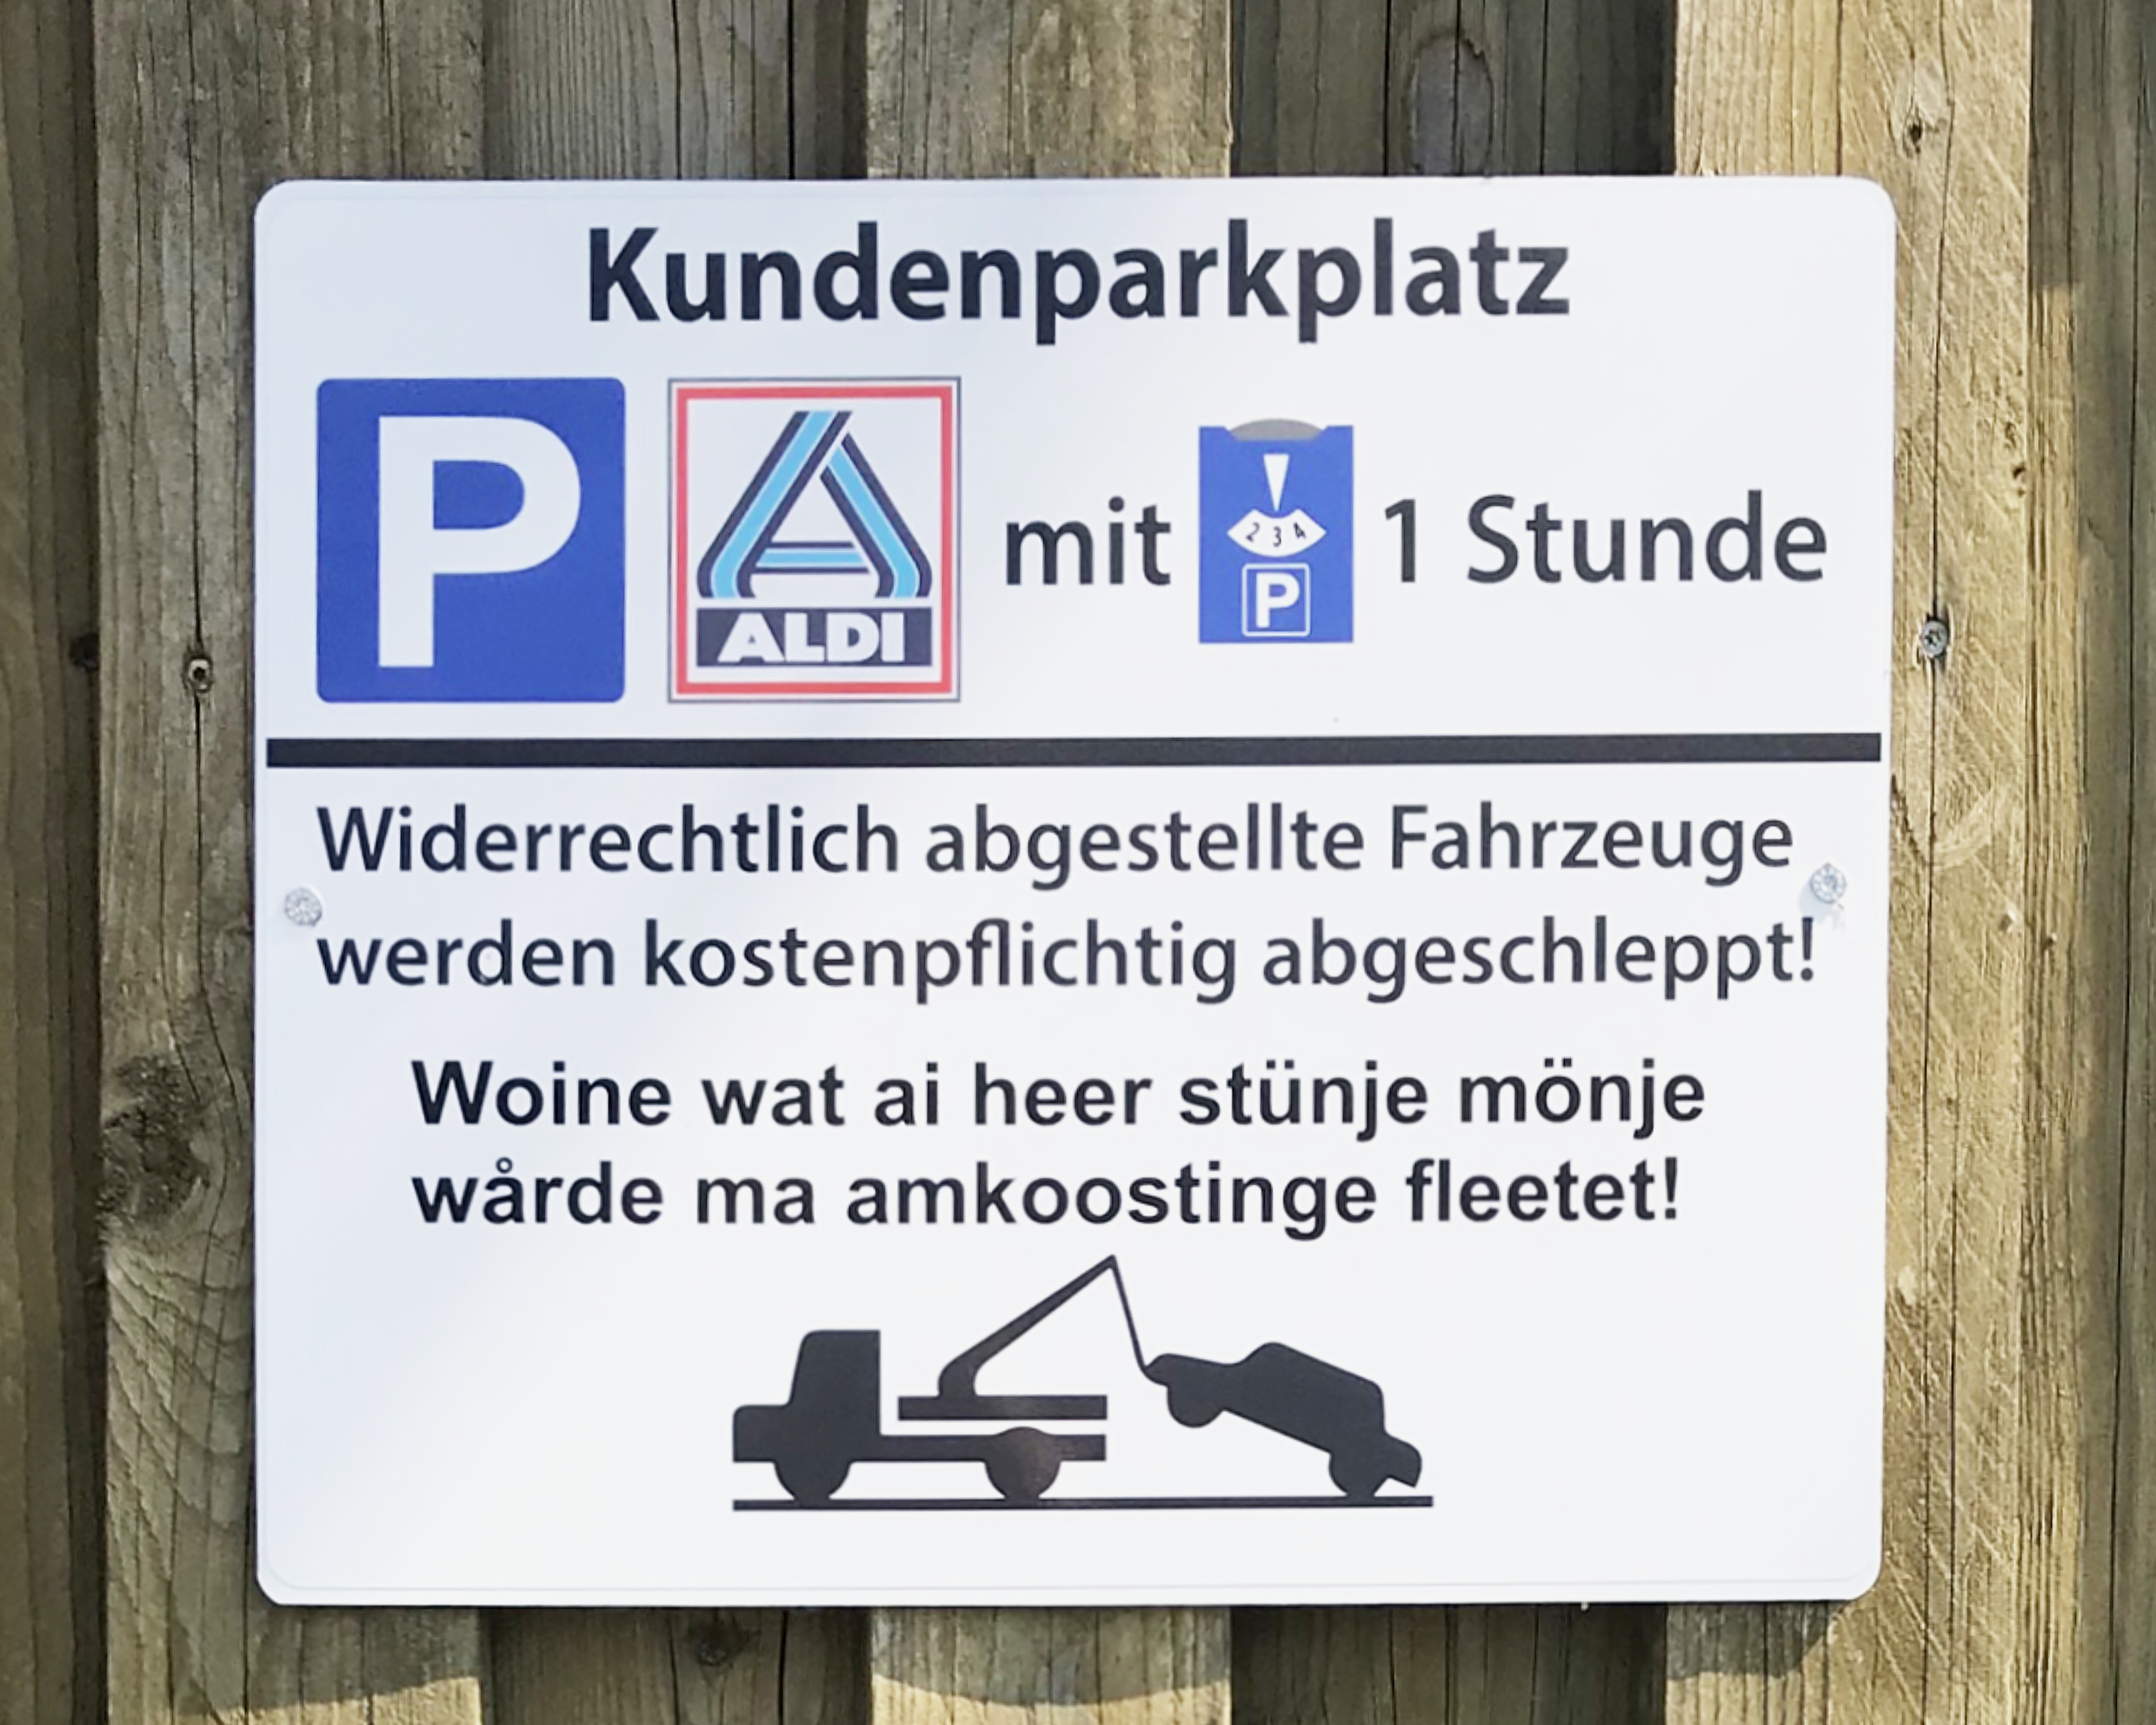
\includegraphics[width=\textwidth]{figures/fig1_gregersen.jpg}
\caption{Sign at the car park of a supermarket in Niebüll (post on a private Facebook wall)}\label{fig:gregersen:1}.
\end{figure}

  
%%please move the includegraphics inside the {figure} environment
%%
 

\begin{figure}
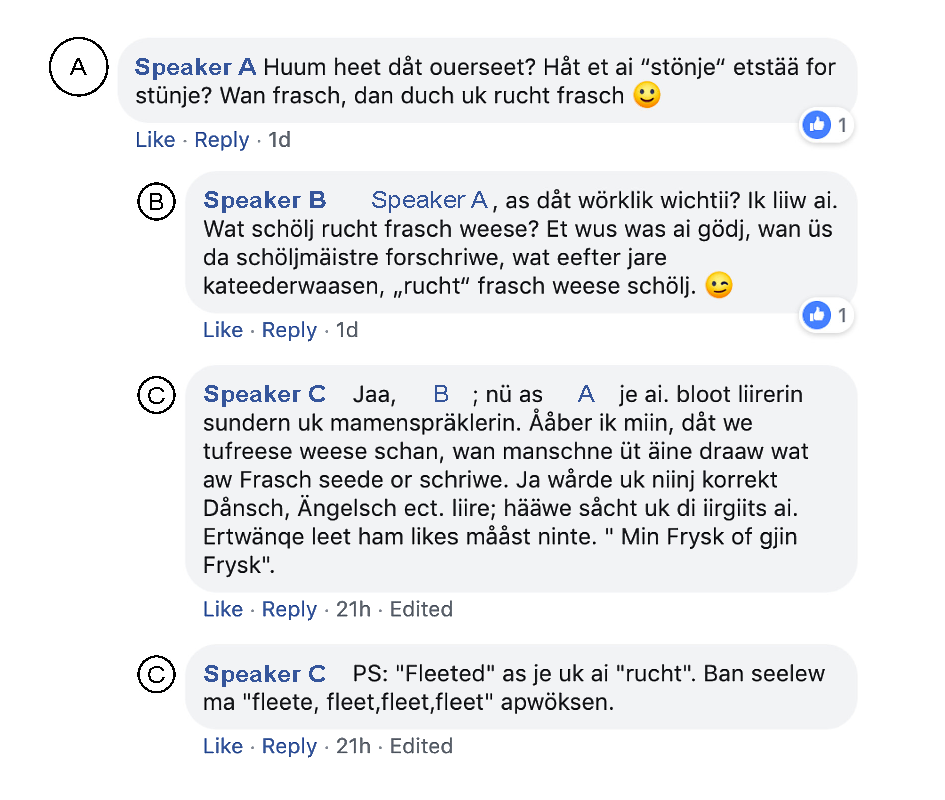
\includegraphics[width=0.8\textwidth]{figures/fig2_gregersen.pdf}
\caption{Caption of and responses to the picture in \figref{fig:gregersen:1} (post on a private Facebook wall).}\label{fig:gregersen:2}
\end{figure}

This picture of the sign was posted on a private Facebook wall with the question in Frisian: ‘Who translated this? Shouldn’t it be \textit{stönje} and not \textit{stünje}?’ This triggered a short trail of responses from the poster’s Facebook friends (see \figref{fig:gregersen:2}), mostly in Frisian, who, incidentally, are all well-known as active members of the Frisian-speaking community. The trigger for their comments relates to the use of \textit{stünje} instead of \textit{stönje} in the translation of \textit{stehen} (‘to stand’, here: ‘to be parked’).\footnote{It was impossible to find out who provided the translation for the car park sign, despite several attempts to contact the manager of the supermarket. \textit{Stönje} is the form listed in the most commonly used dictionary but both forms, \textit{stünje} und \textit{stönje}, are attested in Bökingharde Frisian, with the “incorrect” \textit{stünje} attested for Niebüll, the location of the supermarket, in Walker (1980: 247; with thanks to Temmo Bosse (Flensburg) for helping us find this reference).} We present the beginning of the exchange in translation:

\begin{quote}
A: Who translated this? Shouldn’t it be \textit{stönje} instead of \textit{stünje}? When you use Frisian, it should be correct Frisian [F04A?]
\end{quote}

\begin{quote}
B: A, is this really important? I don’t think so. What is correct Frisian meant to be? It would certainly not be good if our school teachers prescribe, what they, from their vantage point of the pulpit, believe to be “correct” Frisian.   
%%please move the includegraphics inside the {figure} environment
%%\includegraphics[width=\textwidth]{figures/a07GregersenLanger-img003.png}
 
\end{quote}

\begin{quote}
C: Yes, B; but A isn’t just a school teacher but also a native speaker. But I believe that we should be happy [satisfied] when people speak or write something in Frisian of their accord. One wouldn’t ever learn correct Danish or English. And wouldn’t have the ambition to do so, either. You couldn’t force people to do anything anyway. “Bad Frisian or no Frisian.”
\end{quote}

\begin{quote}
C: P.S. “Fleeted’” also isn’t “correct”. I myself grew up with ‘fleete, fleet, fleet, fleet’ [= ablaut forms]. 
\end{quote}

The three commentators are all native speakers of Mainland North Frisian, with speaker A a school teacher of Frisian, speaker B a leading participant in the ethnic and political discourse on the Frisian minority and speaker C a well-known literary scholar and poet of Frisian, who as a student produced an influential dictionary of Mainland North Frisian in the early 1970s. They are all university-educated and take part in writing competitions and/or publish their own short stories and poetry in Frisian but none of them are academic linguists. In this Facebook exchange they argue about the need for using Frasch, their dialect of Frisian, “correctly” especially when it is used in public signage as shown above. A point of controversy in this conversation is the impact of correcting people’s Frisian. It is argued by speakers B and C that not only is it unclear who would have the authority to adjudicate on what is correct but also that being corrected might have the effect that one ceases to speak the language. Speaker C summarizes this succinctly as: better ‘Bad Frisian than no Frisian’, referring implicitly to the book title by \citep{Sjolin1976}, who investigated language mixing in West Frisian.\footnote{\textit{Min frysk} = everyday, spoken language, considered to be a variety of lesser quality; in opposition to the ‘echte Fries’, the real Frisian, used in formal writing \citep[13]{Sjolin1976}.} In subsequent lines of this exchange, not quoted here for the sake of brevity, speaker B re-emphasizes that being a native speaker of Frisian should not be seen as empowerment to correct other people’s Frisian. In response, Speaker A claims to be misunderstood – since they simply had wished to point out that it should have been expected that whoever produced the car park sign would have consulted a native speaker or a dictionary. Speaker B then points out that there is no institution or dictionary for Frisian that provides binding (\textit{ferbindlik}) guidance in such language matters. Speaker B reiterates that it is preferable for people to feel encouraged to write rather than not write at all for fear of making a mistake.

This exchange summarizes some of the key issues in the lay-linguistic discourse on minority languages: in acknowledgement that smaller languages typically do not feature in the public written domain, it is generally applauded when the language is used in linguistic landscapes. However, as soon as there is visible display of the language, issue of language norms and correctness appear: writing has often been reserved only for the most formal, correct or prestigious variety of a language.\footnote{The advent of web 2.0 (the interactive version of the internet) and social media has offered a much-discussed challenge to this doctrine.} In consequence, the expectation of the reader is such that writing in smaller languages will comply with this pattern, given that s/he, like the three speakers in the exchange above, will have obtained their literacy through the medium of a highly codified language, in this case High German. There is the additional tension about who has the authority to say what is correct and what is not. In the exchange, all three refer to two types of norm authorities: on the one hand the judgement of native speakers, and on the other hand the prescriptions provided in reference works. In the case of Mooring, the dialect discussed here, there is a widely-used, explicitly \textit{descriptive} dictionary,\footnote{„By intent and design, the dictionary is descriptive, not normative.’ (\citealt{SjolinEtAl1988}: v; our translation, JG/NL)} that is, however, often perceived to be authorative and sometimes referred to as the \textit{Frisian Duden} (cf. 5.3.2 below), named after the dictionary of German which is commonly perceived to be providing clear judgement on what is German and what is not. 


\subsubsection{The Word of the Week}
\label{sec:gregersen:5.3.2}

The second example is also taken from Facebook but a more public posting, hosted at the facebook page of the \textit{Friisk Foriining}, one of the most active and prominent Frisian cultural associations. For some time, the \textit{Friisk Foriining} has been posting the ‘word of the week’ in order to highlight forgotten words or disappearing words that are of general interest. In early November 2017, the chosen word was \textit{eewensch}, with the following explanation (see \figref{fig:gregersen:3}):

 \begin{figure}
 
\includegraphics[width=\textwidth]{figures/fig3_gregersen}
 \caption{Word of the Week: \textit{Eewensch} (post on Friisk Foriining’s Facebook wall).}\label{fig:gregersen:3}
 \end{figure}



\begin{quote}
Frisian Association
\end{quote}

\begin{quote}
The word of the week.
\end{quote}

\begin{quote}
\textit{Eewensch}
\end{quote}

\begin{quote}
\textit{Eewensch} is a different word for ‘timely, at the same time’. The frequently used word ‘liktidi’ does not really exist in Frisian and has simply been taken from German. […]
\end{quote}

This simple statement started a lively exchange of some 31 comments between the author of the post and a number of commentators, all well-known in the Frisian community, including a university researcher, activists (speaker B and C from the exchange above), and a lecturer from West Frisia in the Netherlands. The key controversy was about the question as to what counts as Frisian. Whilst the initial post condemned \textit{liktidi} to not being Frisian but merely being a German word in Frisian disguise,\footnote{\textit{Liktidi} is plausibly argued to be a morpheme-by-morpheme translation of German \textit{gleichzeitig} (= equal+timely ‘at the same time’).} the first respondent queried this, arguing that since \textit{liktidi} is used by speakers when they speak Frisian, surely it must be a word of Frisian. S/he acknowledges that one may have personal preferences for the use of one word over another but that this does not mean that the dispreferred word is not part of the language:

\begin{quote}
D: Deer fäist tu schüns, dåt än hü ham spräke feranert. Wat ‘hiinj’ än wat ‘gödj’ as, deer koon än schal huum ai am urdiile. Bai ‘eewensch’/‘liktidi’ määst dü et üülj uurd liiwer lise, bai ‘brükd’/’brüked’ määst dü e nai form liiwer lise. 
\end{quote}

\begin{quote}
There you see that language changes. What is “wrong” and what “good” can and should not be judged. With the example of \textit{eewensch / liktidi}, you may well prefer an older word, with \textit{brükd / brüked} [past participle of \textit{brük} ‘to use’\footnote{As part of the exchange, the question of whether \textit{brükd} or \textit{brüked} is the correct participle of \textit{brük} was discussed with similar passion. Here the initial objection to the (more irregular) \textit{brükd} was dropped when a screenshot of the dictionary entry for \textit{brük} was posted.}], you may prefer the younger one. 
\end{quote}

The original author does not accept this. S/he argues that \textit{liktidi} is not a new word of Frisian, it is simply not a word of Frisian, partly because the suffix -\textit{tidi} (‘-timely’) does not exist in Frisian but must have been borrowed from German \textit{{}-zeitig.}\footnote{There is no dispute that \textit{liktidi} is a loan translation from German, so the rebuke here addresses something that hadn’t been suggested.} The author then proceeds by suggesting that if the view of the university people (speaker D works on Frisian linguistics at a university) was that there is no such thing as incorrect (\textit{ferkiird}) or wrong (\textit{hiinj}) Frisian, then there would be quite a gulf between them and us.\footnote{It is not clear what is meant by ‘us’ here, i.e. whether this refers to people speaking Frisian, people working at the Friisk Foriining, or something else.} 

\begin{quote}
FF Liktidi as ai nai, et as iinjfåch niinj frasch. Et jeeft uk niinj uurd ‘tidi’ (aw tjüsch nooch...zeitig). Et as tjüsch, gåns iinjfåch tjüsch. Pjåt wårt duch ai frasch, bloot ouerdåt di spreeger uk wat frasch snååke koon. Wan jam bai e uni önj FL miinje, dåt et niinj ferkiird frasch än uk niinj hiinj frasch jeeft, dan san jam bili wid wach foon üs.
\end{quote}

\begin{quote}
[\textit{Liktidi} is not new, it simply isn’t Frisian. There also isn’t a word \textit{tidi} (though in German there is the equivalent \textit{{}-zeitig}). It is German, plain and simply German. Casual conversation also doesn’t become Frisian just because the speaker knows a little Frisian. If you at the university in FL [i.e. Flensburg] think that there is no such thing as incorrect or ugly Frisian, you are pretty far away from us.]
\end{quote}

The discussion continues in the direction of determining the norm authority for good Frisian. In particular, the role of descriptive dictionaries produced at universities is examined. While some commentators (Speaker B) emphasize that these dictionaries are academic dictionaries and have very little relevance for the speaker community, the author of the weekly column disagrees and states that there is, indeed, a normative reference work – a Frisian \textit{Duden} – , namely the red dictionary by \citet{SjolinEtAl1988}: words included in the dictionary are good Frisian, words that are not included are not good Frisian. The post is closed by the somewhat extraordinary remark that Frisian is a standardized language, not a dialect – straying significantly from the general perception that while Frisian is a language, not a dialect, it is not formally standardized:\footnote{We acknowledge that whilst there is no formal standardization of North Frisian, there is a level of agreement amongst language activists as to what constitutes good grammar, orthography and lexis. Such subsistent norms (cf. \citealt{Gloy1975}) play an important role in the editing of texts in publications, e.g. by the \textit{Nordfriisk Instituut} or the \textit{Ferring Stiftung.}}

\begin{quote}
FF Et jeeft en fraschen ‘Duden’ – dåt as et rüüdj uurdebök foon Sjölin, Walker än Wilts. Wat deerbane stoont as gou frasch, wat ai, dåt ai – sü iinjfåch mååge we üs dåt. Deerfor jeeft et suk referänse. Wan huum miinjt, dåt huum sü schriwe än snååke koon as huum wal, dan schal huum dåt. Hiinj frasch blaft et likes! We as Foriining behoonle frasch as en standardisiirden spräke än ai as en dialekt. Huum miinjt, följk brüket bai frasch nån standard, schååset üüsen spräke! 
\end{quote}

\begin{quote}
[There is a Frisian ‘Duden’ – namely the red dictionary by Sjölin, Walker and Wilts [1988]. What is in there, is good Frisian. What is not in there, is not good Frisian. This is how easily we deal with the problem. This is why such reference works exist. If anyone thinks they can write or speak as they wish, they should do so. This does not alter the fact that it is ugly Frisian. We at the Friisk Foriining consider Frisian a standardized language and not a dialect. If anyone thinks that the people don’t need a standard for Frisian, damages our language.]
\end{quote}

This exchange continues back and forth a little longer. The principal discord relates to the importance of maintaining a standard so as to protect the language from disintegration and to the potentially damaging effect of policing or correcting people when they speak Frisian, especially those who are native speakers. It demonstrates the level of conviction that most contributors have when it comes to postulating or confirming that there is a correct way of speaking Frisian, that it is crucial for the existence of Frisian to have such a standard, and that the language requires active support to maintain its distinctiveness. Incidentally, what is missing in these discussions are the voices of those native speakers who are not active in any metalinguistic debates (cf. \citealt{AdmiraalEtAL2019} for ways of redressing this imbalance). 

\section{Conclusion}
\label{sec:gregersen:6}

This book discusses the issue of language contact from a number of perspectives. This chapter focuses on the \textit{perception} of language contact, in particular the evaluation of language contact in the context of threatening or damaging the linguistic integrity of the receiving language. It is well-known that discourses of language decay can be found for many languages and that such decay is often seen to be caused by two factors: careless use of the language (not pronouncing endings, not using synthetic case markings, etc.) and use of foreign borrowings instead of indigenous lexis and morphology. However, in academic circles amongst linguists of bigger languages, such concerns are not part of a scholarly engagement with language change: change is considered to be cost-neutral, i.e. whilst the language looks different after a particular change has happened, it is not \textit{qualitatively worse} in its ability to serve as a communicative tool to express the thoughts of its speakers. Discourse on language decay in bigger languages is driven by the concerns of those without a formal training in linguistics or by those who openly embrace a standard-language ideology.\footnote{Cf. the current debate amongst scholars of German on pluriareal vs. pluricentric languages, a debate which is also fought in the perception of some that a national variety such as Austrian German would suffer in prestige if it were not afforded the status of a national standard language (cf. \citealt{Dollinger2019} for one controversial side of the argument).} Such a division is less clear for minority-language linguistics. This chapter provided evidence from three types of discourse to show that when it comes to smaller languages, i.e. those that are in long-lasting contact with a majority language, the discourse of language decay through neglect and external influence is not restricted to non-academic linguists. Instead it is acceptable in the field not only to engage in codificatory processes (production of dictionaries and grammars; teaching material) but also to voice concerns about changes in the languages: such changes are almost exclusively attributed to external influences and are rarely viewed neutrally. Language change, in particular change through language contact, is considered to be damaging to the linguistic system and lexis of the smaller language. This is all the more striking as particular doctrines such as “all languages have always changed and will always change” are still upheld, despite the tension they invoke in connection with views of language change as decay and language contact as a threat.\footnote{As \citet{AdmiraalEtAL2019} have shown, such views, i.e. that language contact is a problem or a threat, are not universally shared amongst \textit{native speakers} of smaller languages; they also show that there are individuals and groups who simply note results of contact such as borrowing or syncretism as part of their language(s). However, such views are never heard in the public discourse on the state of Frisian but remain restricted to those who are not part of the scholarly discourse.}

\section*{Acknowledgements}

We are grateful to Nils Århammar (Bräist), Temmo Bosse (Flensburg), Jarich Hoekstra (Kiel), Samantha Litty (Flensburg), Lena Terhart (Flensburg), the editors of this volume and the anonymous reviewers for their critical comments and helpful corrections. All remaining errors are, of course, solely the responsibility of the authors.


{\sloppy\printbibliography[heading=subbibliography,notkeyword=this]}
\end{document} 
